\section{Bayesian regression trees}\label{section:Model}

In this section, we describe how we adapt the Bayesian Additive Regression Trees (BART) prior \citep{BARToriginal} to high-dimensional covariates by introducing a horseshoe prior on the step heights.
This approach shifts regularisation from the tree structure (e.g. \citet{linero2018dirichlet}) to the step height parameters.
We start with an overview of how BART is applied to model log survival times under the accelerated failure time (AFT) framework.
We detail our novel adaptation using a global--local shrinkage prior.
We then explain how the model accommodates censored outcomes.
Finally, we discuss default hyperparameter choices.


\subsection{Overview of Bayesian Additive Regression Trees (BART)}

We adapt the BART model to estimate the conditional mean function $\mathbb{E}[\log{T_i}\mid X_i = x]$ in the AFT model.
The uncensored survival times are modelled as a noisy sum of trees:
\begin{equation}\label{bart_model}
\log{T_i} = \sum_{j=1}^m g(X_i; \mathcal{T}_j, \mathcal{H}_j) + \varepsilon_i, \quad \varepsilon_i \sim \mathcal{N}(0, \sigma^2),
\end{equation}
where each $\mathcal{T}_j$ is a binary decision tree that defines recursive partitioning rules over the covariate space, and $\mathcal{H}_j = \{h_{j1}, \ldots, h_{jL_j}\}$ denotes the set of step heights associated with the $L_j$ leaves of tree $\mathcal{T}_j$.
We extend this model to accommodate censored survival times in Section~\ref{cens_bin}.

The function $g(x; \mathcal{T}_j, \mathcal{H}_j)$ maps $x$ to a leaf node $\ell$ in $\mathcal{T}_j$ and returns the corresponding value $h_{j\ell}$. 
Each tree partitions the covariate space into disjoint regions, assigning a constant prediction to each region (see Figure~\ref{ExampleTree}).


\begin{figure}[tb]
    \centering
    \begin{minipage}{.5\linewidth}
      \centering
      \begin{tikzpicture}[
            box/.style={rectangle, draw, rounded corners, align=center, minimum height=10mm, minimum width=16mm},
            leaf/.style={circle, draw, align=center, minimum size=10mm},
            line/.style={-latex}
        ]
        
        % Root node
        \node [box] (root) {$x_1 < 0.7$};
    
        % Level 1 nodes
        \node [box, below=1cm of root, xshift=-2cm] (left) {$x_2 < 0.6$};
        \node [leaf, below=1cm of root, xshift=2cm] (h1) {$h_1$};
    
        % Level 2 nodes
        \node [leaf, below=1cm of left, xshift=-1cm] (h2) {$h_2$};
        \node [leaf, below=1cm of left, xshift=1cm] (h3) {$h_3$};
    
        % Draw edges with labels
        \draw[line] (root) -- (left) node[midway, above left] {Yes};
        \draw[line] (root) -- (h1) node[midway, above right] {No};
        \draw[line] (left) -- (h2) node[midway, above left] {Yes};
        \draw[line] (left) -- (h3) node[midway, above right] {No};
    
        \end{tikzpicture}
    \end{minipage}%
    \begin{minipage}{.5\linewidth}
      \centering
      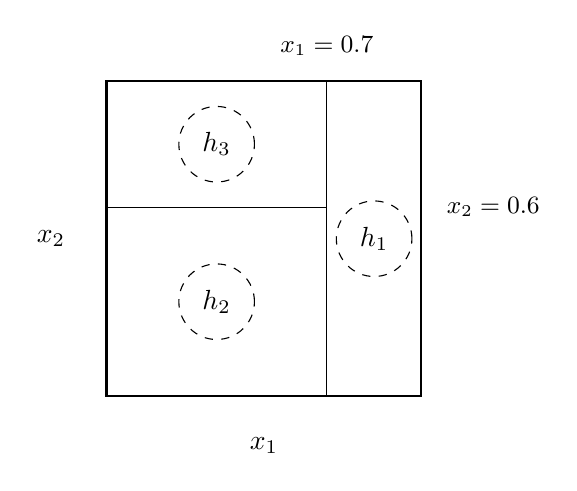
\begin{tikzpicture}[scale=4] % Increase scale for a larger square
            % Define the unit square
            \draw[thick] (0, 0) rectangle (1, 1);
            
            % Vertical line at x1 = 0.4
            \draw[thin] (0.7, 0) -- (0.7, 1) ;
            
            % Horizontal line at x2 = 0.7
            \draw[thin] (0, 0.6) -- (0.7, 0.6);
            
            % Labels for axes
            \node[below] at (0.5, -0.1) {$x_1$};
            \node[left] at (-0.1, 0.5) {$x_2$};
    
            % Splitting variables of the partition
            \node[right] at (1.05, 0.6)  {\small{$x_2 = 0.6$}};
            \node[above] at (0.7, 1.05)  {\small{$x_1 = 0.7$}};
            
            % Step heights
            \node at (0.85, 0.5) {$h_1$};
            \node at (0.35, 0.3) {$h_2$};
            \node at (0.35, 0.8) {$h_3$};
    
            % Circles arounnd 
            \draw[dashed] (0.85, 0.5) circle [radius=0.12];
            \draw[dashed] (0.35, 0.3) circle [radius=0.12];
            \draw[dashed] (0.35, 0.8) circle [radius=0.12];
            
        \end{tikzpicture}
    \end{minipage}
    \caption{Example of a decision tree with the corresponding partition of the covariate space $[0,1]^2$ and the associated step heights $\H = \{h_1, h_2, h_3\}$.}
    \label{ExampleTree}
\end{figure}



We place an independent prior on each tree $(\mathcal{T}_j,\mathcal{H}_j)$ in the ensemble.
The prior factorises as $p(\mathcal{T}_j,\mathcal{H}_j)=p_{\mathcal{T}}(\mathcal{T}_j)\,p_{\mathcal{H}}(\mathcal{H}_j\mid \mathcal{T}_j)$ for $j=1,\ldots,m$.
The structure prior $p_{\mathcal{T}}$ is specified as a heterogeneous Galton--Watson branching process \citep{TheoryBART}. 
Conditionally on $\mathcal{T}_j$, standard BART assigns independent Gaussian priors to the step heights, $h_{j\ell}\sim \mathcal{N}\!\left(0,1/(4\sqrt{m})\right)$. 
The scaling is chosen so that the induced prior on the sum of trees places most mass within the observed response range.
This conjugate choice enables efficient Gibbs updates. 
We modify this prior to accommodate continuous shrinkage of the step height parameters.


\subsection{Horseshoe prior on the step heights}\label{stepheight_prior}

% Setup: introduce prior structure for step heights using scale mixtures
We present our novel formulation of step height prior based on a global--local shrinkage prior.
Given a tree $\T$ with $L$ leaf nodes, we specify a prior on the set of step heights $\H = \{h_1, h_2, \dots, h_L\}$.
To achieve shrinkage in high-dimensional covariate spaces, we use a class of continuous shrinkage priors on the set of step heights. 
This class can be represented as a scale mixture of normal distributions.
In general form, the prior $p_\mathcal{H}$ is specified hierarchically:
\begin{equation}
\begin{split}
h_\ell \mid \lambda_\ell^2, \tau^2,  \omega &\sim \mathcal{N}(0, \omega \lambda_\ell^2 \tau^2), \\
\lambda_\ell^2 &\sim p(\lambda), \\
\tau^2 &\sim p(\tau),
\end{split}
\end{equation}
where $\ell = 1, \ldots, L$, and $\omega$ is a fixed hyperparameter that ensures appropriate scaling of the prior variance relative to the tree-based model structure.

% horseshoe instantiation: define the Horseshoe using half-Cauchy priors
The horseshoe prior \citep{OriginalHorseshoe, PolsonScott2011} arises by specifying half-Cauchy distributions for both the global and local shrinkage parameters:
\begin{equation}\label{Horseshoe}
    \tau \sim \mathcal{C}^+(0, \alpha_\tau) \quad \text{and} \quad \lambda_\ell \sim \mathcal{C}^+(0, \alpha_\lambda) \ \text{ for } \ \ell = 1, \ldots, L,
\end{equation}
where $\mathcal{C}^+(0, \alpha)$ denotes the half-Cauchy distribution with location zero and scale parameter $\alpha > 0$.
Note that the median of the distribution equals $\alpha$, while the mean and variance do not exist due to the heavy tails.
We refer to this specification of the prior as a \textsl{Horseshoe Forest}.
A Horseshoe Forest refers specifically to a single learner for the outcome, as in~\eqref{bart_model}.
In contrast, the \textsl{Causal Horseshoe Forest} decomposes the outcome into a prognostic function and a treatment effect function (see~\eqref{model}), each modelled by its own Horseshoe Forest.

% Interpretation: explain global--local roles and behaviour of shrinkage in trees
This formulation falls within the class of global--local shrinkage priors \citep{PolsonScott2011}. 
The \textit{global shrinkage parameter} $\tau$ governs the overall degree of shrinkage, encouraging all step heights to be small, while the \textit{local shrinkage parameters} $\lambda_\ell$ allow individual step heights $h_\ell$ to deviate from this global tendency when supported by the data. 
In the tree-based context, the local shrinkage parameters refer to the values assigned to individual leaf nodes, each associated with a distinct region of the covariate space, whereas the global shrinkage parameter is shared across all leaf nodes. 
This hierarchical structure enables the model to suppress noise in regions lacking signal while preserving flexibility in regions where effects are present. 
The horseshoe prior is particularly well-suited for this task, as it can adapt to varying degrees of sparsity without imposing excessive shrinkage on substantial signals \citep{vdPas2017, vdPas2017Horseshoe, bhadra2019lasso}.

% Specification global shrinkage parameter
The global shrinkage parameter $\tau$ can be specified either as a single parameter shared across the entire forest or assigned separately per tree.
We adopt the latter approach and assign a separate global shrinkage parameter to each tree. 
This choice is motivated by two considerations. 
First, assigning independent global shrinkage parameters preserves the prior independence between trees.
While the trees are not independent in the posterior due to their shared dependence on the residuals, this prior structure encourages each tree to act as a weak learner, consistent with the additive ensemble construction underlying boosting-type methods.
Weak learners have limited individual accuracy and are combined to form a strong ensemble learner \citep{Schapire1990WeakLearnability, Freund1997Boosting}.
Second, each tree partitions the covariate space differently and may focus on distinct regions with varying signal strength. 
A shrinkage parameter shared across the forest would force the same level of regularisation across the entire covariate space.
This would be inefficient in heterogeneous settings.
Tree-specific shrinkage allows the model to adapt locally: it can apply more shrinkage in noisy regions and less in informative ones.


% Shrinkage vs selection: motivate shrinkage for causal inference vs model selection
We prefer continuous shrinkage over exact sparsity in high-dimensional causal inference.
Model selection methods like LASSO-based methods \citep{Belloni2014, Shortreed2017} or DART \citep{linero2018dirichlet} induce sparsity by forcing some coefficients to be exactly zero, whereas shrinkage priors such as the horseshoe continuously pull estimates toward zero without fully excluding the respective covariates. 
This distinction is particularly relevant in causal settings, where omitting covariates risks violating the unconfoundedness assumption (see \eqref{unconfoundedness}).

% Conceptual connection: trees as averaging over normal means models
From a conceptual perspective, the use of continuous shrinkage priors in tree-based models is also supported by their connection to the classical normal means problem \citep{james1961estimation}. 
If the covariate space were partitioned into $n$ leaf nodes, each containing a single observation, the model would reduce to a set of independent normals centred at the leaf-specific means. 
Although such fine partitions are unlikely under the prior, the Bayesian tree ensemble can be viewed as performing Bayesian model averaging over normal means models that cluster observations based on covariate similarity.
This connection also supports recent advocacy for Bayesian model averaging in causal inference \citep{Wang2012, Zigler2016, Horii2021BMA, Antonelli2020Averaging}.
This perspective becomes explicit in Section~\ref{subsection:full_conditional}, where we describe a full conditional posterior draw of the step height parameters. 



\subsection{Choice of hyperparameters}\label{default_hyperparameters}
We follow the default recommendations of \citet{BARToriginal} regarding the hyperparameters governing the prior on the tree structure. 
Empirical evaluations suggest that the influence of these parameters is negligible in our setting. 
We set the number of trees to 200 for both the prognostic and treatment effect forests. 
This contrasts with the recommendation of \citet{hahn2020bayesian}, who advocate using a smaller number of trees for the treatment effect model as a form of regularisation. 
In our approach, regularisation is instead achieved through the prior on the step heights. 
We have found that using a larger number of trees, which induces a finer partition of the high-dimensional covariate space, improves estimation in this context.

We adopt an empirical approach to set the prior hyperparameters, following the recommendation of \citet{BARToriginal}. 
Specifically, we centre and standardise the log-transformed survival times using preliminary estimates of the mean and variance, obtained either from a linear AFT model for high-dimensional data \citep{Kumari2025afthd} or from an intercept-only AFT model. 
For the Horseshoe Forest model, which uses a single forest, we set the variance scaling parameter to $\omega = 1$. 
In the Causal Horseshoe Forest model, where the outcome is modelled as the sum of two forests for $f(x)$ and $\tau(x)$, we set $\omega = \frac{1}{2}$ to ensure that sufficient prior mass is allocated across the observed outcome range. 


The global and local shrinkage parameters $\tau$ and $\lambda$ are assigned half-Cauchy priors with scale parameters $\alpha_\tau$ and $\alpha_\lambda$, respectively. 
For simplicity, we set $\alpha := \alpha_\tau = \alpha_\lambda$. 
Some studies recommend using a different prior scale for the global parameter $\tau$ than for the local parameters $\lambda_\ell$ to better control overall shrinkage \citep{Piironen2017Hyperprior}. 
In our experiments, we found that setting the same scale for both worked well in practice.
This fully Bayesian specification remains adaptive and robust across various settings.
We parametrise the scale as $\alpha = \frac{k}{\sqrt{m}}$ for some $k > 0$, where $m$ denotes the number of trees in the respective forest. 
The choice of $k$ governs the level of shrinkage.
We recommend setting $k = 1$ for conservative shrinkage, $k = 0.1$ for moderate shrinkage, and $k = 0.05$ for more aggressive shrinkage. 
At the start of the chain, a small value for $k$ prevents the sampler from becoming trapped in local regions. 
As the chain converges toward its stationary distribution, the heavy-tailed nature of the horseshoe prior allows the posterior to explore the full parameter space. 
In practice, we recommend selecting $k$ via cross-validation.
We perform cross-validation for censored data using the concordance index (C-statistic) \citep{harrell1982evaluating}, computed on held-out test predictions.


\subsection{Censored and binary outcomes}\label{cens_bin}

We account for censoring through data augmentation within the Gibbs sampler \citep{TannerWong1987}. 
Censored event times are treated as latent variables and sampled from their full conditional posterior distributions at each iteration. 
We adopt this strategy in both the Horseshoe Forest and Causal Horseshoe Forest to account for censoring in survival outcomes.

The model also supports binary outcomes.
We follow the probit approach of \citet{BARToriginal}, which uses a latent Gaussian variable linked to each binary response.
This latent variable is modelled as a sum of trees, using the data augmentation scheme of \citet{AlbertChib1993}.
We implement this binary extension only for the Horseshoe Forest and use it to estimate the propensity score.